% Chapter 3

\chapter{The Fermilab Muon g-2 experiment} % Main chapter title

\label{Chapter3} % For referencing the chapter elsewhere, use \ref{Chapter3} 

\section{The Fermilab Muon g-2 Experiment}

A description of the muon beam preparation and its delivery into the experiments storage ring will be explained. Information on the major components of the Fermilab muon g-2 experiment will be described. The tracking detectors will be discussed briefly here and described in detail in chapter 5.

\section{Production and preparation of the muon beam}

The muon campus at Fermilab produces high purity $\sim$ 95$\%$ muon bunches. The entire muon campus is illustrated in figure 4.1. The process of creating these bunches starts with the Booster. This increases the energy of the delivered 400 MeV protons into 8 GeV protons. Within the booster, for each 1.4s cycle of the accelerator, four bunches of 8 GeV protons are produced. These are then injected into the Recycler ring through the Main Injector (MI) line. Here each bunch is further divided into four. These sub-bunches contain ~$10^{12}$ protons and must have a temporal length shorter than the cyclotron frequency of 149 ns. The compacted sub-bunches are concentrated at the beginning of the MI cycle, which are separated by 10 ms due to data aquisition limiting the time between pulses. Where the average fill rate is approximately 12 Hz. Figure 4.2 shows the structure of the proton beam pulses.

\begin{figure}[th]
\centering
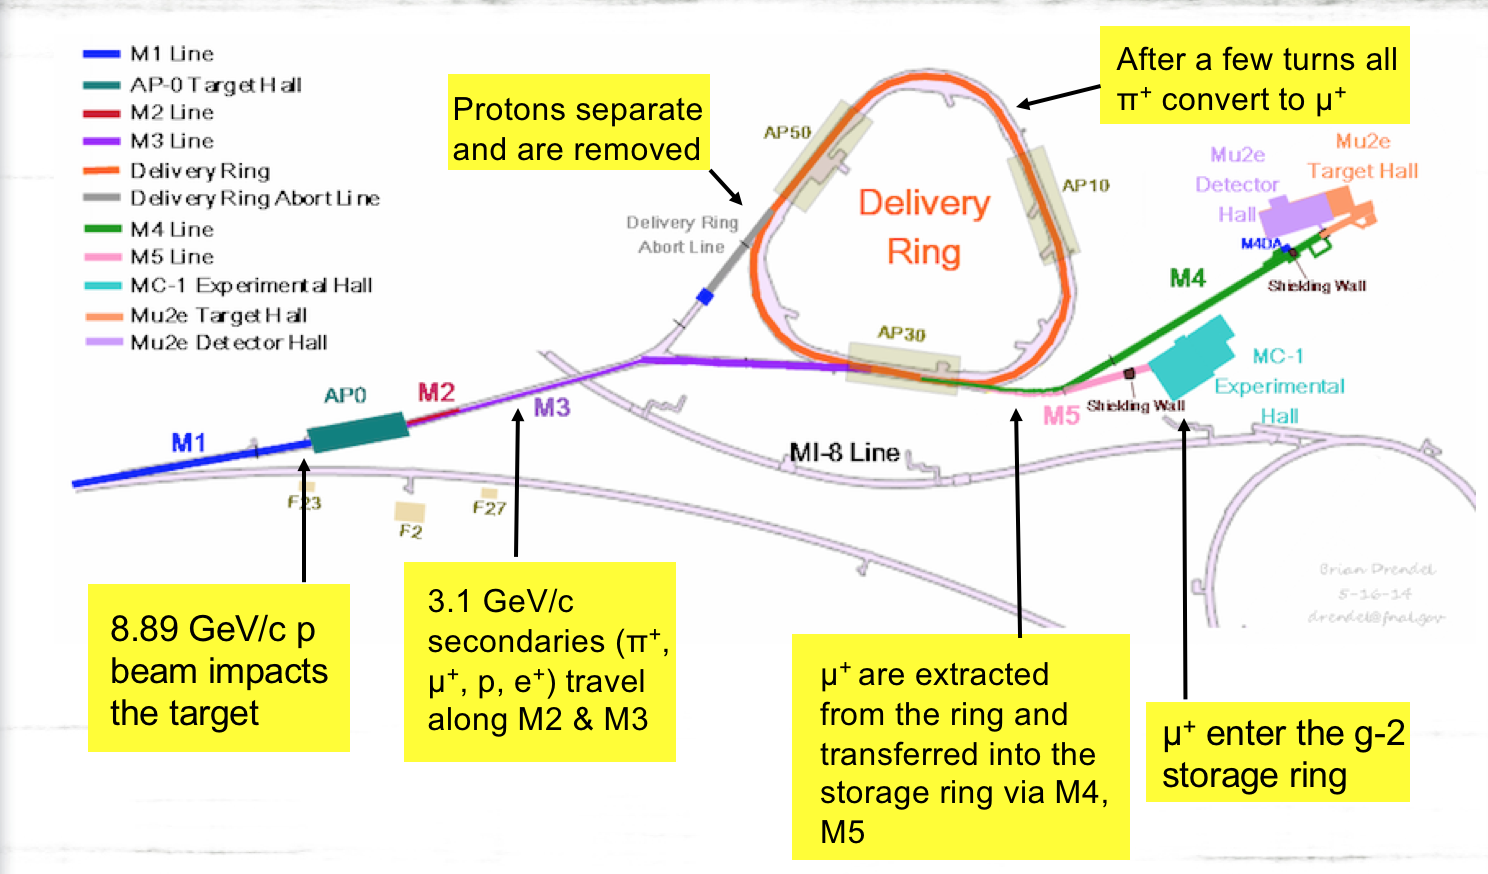
\includegraphics[scale=0.45]{Figures/muonbeamproduction}
\decoRule
\caption{The muon campus layout for muon beam production}
\label{fig:muonbeamproduction}
\end{figure}

\begin{figure}[th]
\centering
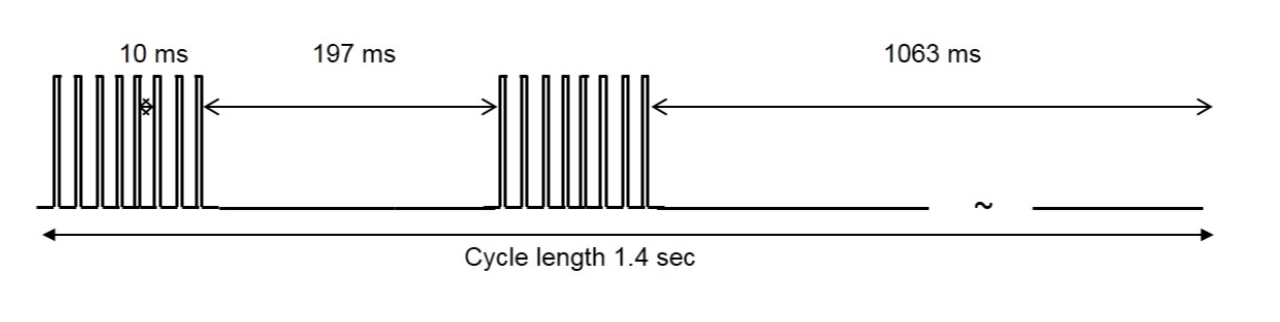
\includegraphics[scale=0.6]{Figures/beampulses}
\decoRule
\caption{Time structure of beam pulses}
\label{fig:beampulses}
\end{figure}

The bunches are then directed separately through the P1,P2 and M1 lines and directed at the Target station which is located in the AP0 hall. Each bunch of 8 GeV protons are fired separately at the pion production target, with the beam parameters at this position shown in Table 4.1. The positively charged particles produced are momentum selected to 3.11 GeV/c $\pm 10\%$ by use of a pulsed dipole magnet and collimator. The beam is then directed through the M1 and M2 lines which select muons produced from the pion decays with a momentum of 3.094 GeV/c. Particles that are not momentum selected will continue forward and be absorbed into the target vault beam dump \cite{Chap2Ref1}.


\begin{table}[th]
\centering
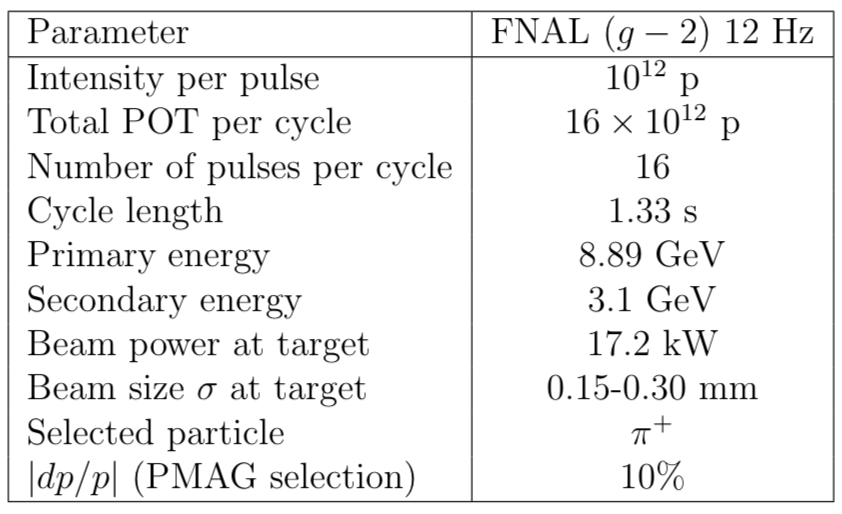
\includegraphics[scale=0.5]{Figures/BeamParameters}
\decoRule
\caption{Beam parameters at the Target station \cite{Reference29}.}
\label{fig:BeamParameters}
\end{table}

The remaining muons are directed into the delivery ring along with any remaining protons and pions. The beam circulates around the delivery ring four times, by which time all pions should have decayed. Any remaining protons are removed by a kicker since they travel slower than muons and become separated from the muon bunch. This produces an approximately 95$\%$ pure polarised muon beam. The beam is then guided into the M4/M5 beamline to the MC1 experimental hall. Here final focusing is provided by magnetic quadrupoles before the muon beam enters the storage ring through the inflector \cite{Reference22}. 

\begin{figure}[th]
\centering
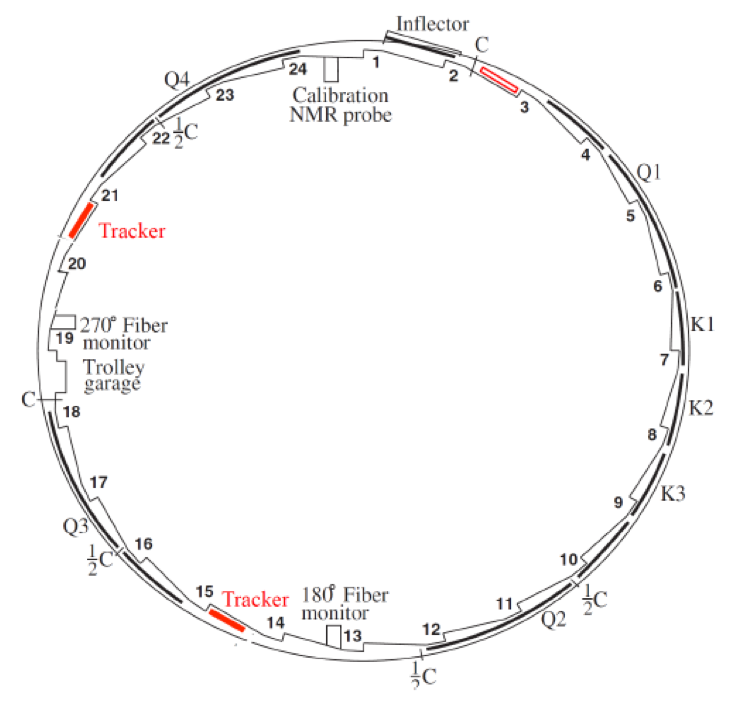
\includegraphics{Figures/ringcomponents}
\decoRule
\caption{Diagram of the storage ring and its main components. The kicker positions indicated by a "K", the collimators with a "C", the quadrupole positions with a "Q",the tracking stations placed at 180$^\circ$ and 270$^\circ$ and the 24 calorimeter locations around the ring.}
\label{fig:ringcomponents}
\end{figure}

\section{Injection into the storage ring}

The polarised muon beam is injected into the storage ring as shown in figure 4.3. To do this it must pass through the storage ring magnetic field. However doing this would deflect the path of the muons and cause them to exit the storage ring. To counteract this effect the inflector which is a 1.7 m superconducting magnet is placed at the point of injection to create an almost magnetic-field-free region. The inflector makes a 1.5 T uniform vertical field which acts to cancel out the storage ring magnetic field and allow the muon beam to pass into the storage ring mostly unperturbed. The inflector was constructed such that its own magnetic field does not affect the highly precise sub-ppm level storage ring magnetic field.

\begin{figure}[th]
\centering
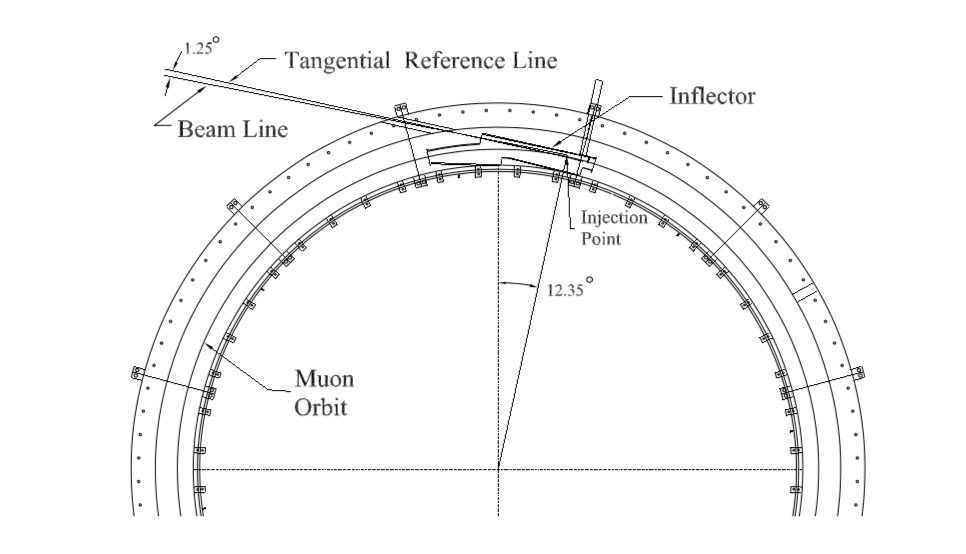
\includegraphics[scale=0.9]{Figures/injectionbeamline}
\decoRule
\caption{Diagram of the beam entering the storage ring.}
\label{fig:injectionbeamline}
\end{figure}

Muons are delivered to the storage ring in 120 ns pulses at an average rate of 12 Hz. Every muon bunch forms one fill of more than 6000 muons. The beam line leading to the inflector is positioned at a 1.25$^{\circ}$ angle from the tangential direction to allow the beam to enter the inflector almost parallel to it. A layout of this is shown in figure 4.4. The position at which the beam enters the storage ring through the inflector is at a circumference 77 mm radially larger than the muon magic radius. 

To direct the muon bunches onto the magic radius a device called the kicker system is used. The kicker system is comprised of three independent 1.27 m long plate magnets. This system is placed at approximately 90$^{\circ}$ around the ring after the injection point, at the position where the muons orbit intersects with the muon magic radius. The beam bunch crosses the muon magic radius at an angle of $\theta_{0}$= 10.8 mrad, 90$^{\circ}$ around the ring. The kicker produces outward 0.03 T transverse magnetic field pulses. These last the entire bunch width of 120 ns to create a 10.8 mrad angular kick that directs the muons onto the ideal orbit. Immediately after the kicker pulse must lower to zero before the bunch returns to the same position 149 ns later.

The kicker device resides within the precision magnetic field. Consequently the kicker cannot consist of any magnetic materials which would perturb the magnetic field. The kicker does not direct all muons exactly onto the magic radius as there is a small momentum spread in the muon beam which results in a slight spread in the beam distribution.

As the muon beam orbits the storage ring, its distribution will spread out vertically and pass outside the storage orbit region. Electrostatic quadrupoles are used to provide vertical focusing. Four electrostatic quadrupoles are placed symmetrically around the ring to produce four separate regions of focusing. In an ideal situation the electrostatic quadrupoles would be placed throughout the whole ring circumference but the inflector, kickers and spaces for the tracking detectors produces four gaps and instead provides 43$\%$ coverage of the ring circumference.

Electrostatic quadrupoles were chosen for vertical focusing rather than magnetic quadrupoles in order to not perturb the storage ring magnetic field. The quadrupole field acts to focus the beam vertically while defocusing the stored beam radially. However the combined effect of the radial electric field and the vertical storage ring magnetic field provides radial focusing. This leads the storage ring to behave as a weak focusing betatron.

There are collimators placed around the storage ring, these are Copper rings with an inner radius of 45 mm which are used to remove muons which lie outside the 9 cm diameter muon storage region. The collimators can either be rotated into position at the storage ring region during data taking or removed from the storage region to allow for NMR trolley runs to map the magnetic field in the storage region. The electrostactic quadrupole plates are charged asymmetrically which moves the beam horizontally and vertically to direct the outliers towards the collimators where they lose energy and are lost after several orbits. This process is called scraping. It begins at 8 $\mu{s}$ after beam injection and continues for 5 $\mu{s}$. Once scraping is completed, the quadrupole plates are charged symmetrically to enable vertical beam storage. The removal of the muons lying at the extremities results in a reduction in the momentum spread of the stored beam to 0.15$\%$.

\section{Positron decay in the storage ring}

For a muon traversing the storage ring at the magic momentum, its time dilated lifetime increases from a rest lifetime of 2.2 $\mu$s to 64 $\mu$s. With a cyclotron frequency of 149 ns, muons will circulate the storage ring numerous times before their decay. This means that the lifetime of the muon is long enough for the observation of multiple oscillations of the anomalous precession frequency $\omega_{a}$ which has a time period of 4.4 $\mu$s.

\begin{figure}[th]
\centering
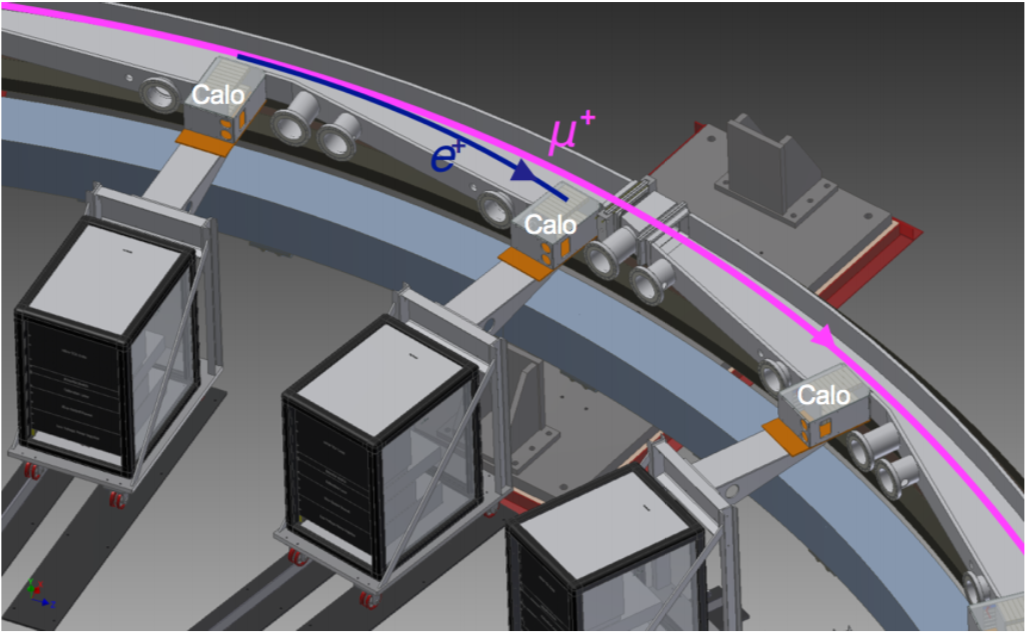
\includegraphics[scale=0.7]{Figures/positronDecay}
\decoRule
\caption{Trajectory of a decay positron following the decay of an orbiting muon \cite{Reference29}}
\label{fig:positronDecay}
\end{figure}

The decay positrons are Lorentz boosted and thus are emitted predominantly along the muon momentum direction. The high energy decay positrons observed by the detectors are emitted within 2$\%$ of the muons momentum direction. This means that the decay positrons accepted by the detectors are approximately tangential to the muon beam orbit. During muon decay, energy is lost to neutrinos and thus the decay positron has lower momentum than the muon. Therefore the positron has a more curved trajectory in the magnetic field at a smaller radius than the muon. Hence the positrons path will travel radially inwards towards the centre of the storage ring, where the detectors are located for measurement as shown in figure 4.5. Data is taken for approximately 650 $\mu$s, by which time the majority of muons will have decayed. 

\section{The magnetic storage ring}

\begin{figure}[th]
\centering
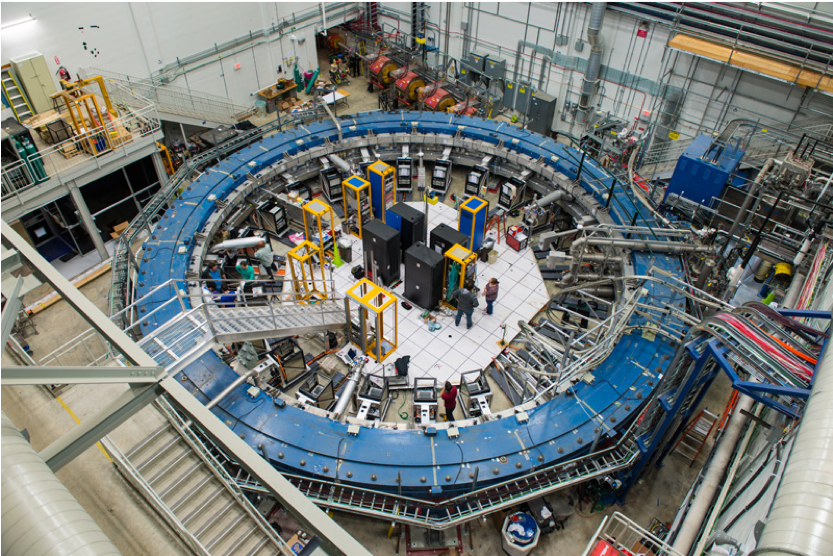
\includegraphics{Figures/storagering}
\decoRule
\caption{Photograph of the muon g-2 storage ring which reuses the BNL 1.45 T storage ring.}
\label{fig:storagering}
\end{figure}

The calculation of a$_{\mu}$ requires a precise measurement of the magnetic field sampled by the muon beam distribution along with a precise measurement of $\omega{_a}$. 
To enable this precision to be achieved the magnetic field located in the muon storage radius needs to be extremely uniform and stable over time to obtain a precise magnetic field map.
 
The goal of the Fermilab E989 experiment is to determine the magnetic field averaged over time in the beam storage region to an uncertainty of $\pm$70 ppb, an improvement from the 170 ppb at BNL \cite{Reference22}. This experiment will reuse the magnetic storage ring originally designed and constructed for the Brookhaven muon g-2 experiment, as seen in figure 4.6. The 15 m diameter superconducting coils required specialist transportation and were shipped from BNL to Fermilab in one piece to reduce the damage inflicted on the precision magnetic field. Other components including the pole pieces and steel yoke were separated and transported individually to be reassembled at Fermilab \cite{magref2}. A diagram of the muon g-2 magnet is shown in figure 4.7.

\begin{figure}[th]
\centering
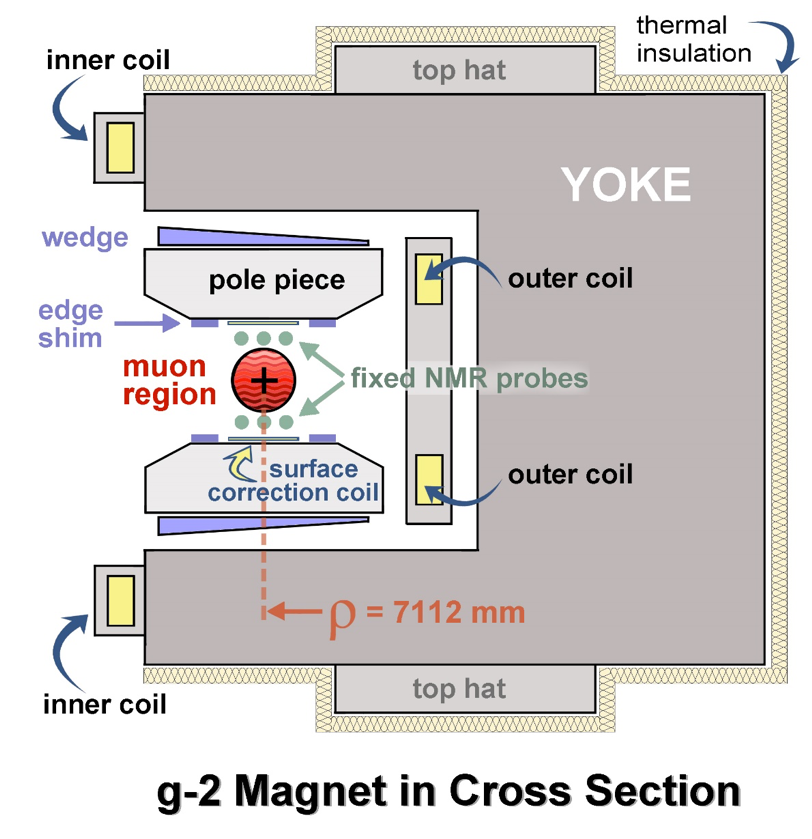
\includegraphics[scale=0.8]{Figures/storageringmagnet}
\decoRule
\caption{Diagram of the cross section of the storage ring. 
Showing the location of the muon storage region and locations of the fixed probes. It also shows the superconducting magnet components including the yoke, coils and pole pieces.}
\label{fig:storageringmagnet}
\end{figure}

The iron dipole magnet is designed to produce a vertical uniform beam of 1.451 T, with a uniformity of 1 ppm when averaged over the full azimuth of the storage ring. The continuous magnet yoke is constructed from a dozen $\ang{30}$ sections of iron. Each section containing an upper and lower yoke which are separated by a spacer plate. The storage ring is approximately 3 m tall, 15 m in diameter, weighs over 700 tons and has a ideal muon storage radius of 7.112 m.  

This dipole magnet is excited by three superconducting Niobium-titanium (NbTi) coils placed above and below the storage region which create the magnetic field\cite{magref3}. Iron pole pieces are placed in between the superconducting coils to create a uniform dipole field. The magnetic field is produced with a current of 5176 A through the superconducting coils. To cool the superconducting coils to the required temperature a cryogenic system is used. Two of the superconducting coils sit at a radius of 6677 mm with the third placed at 7512 mm. The current in the coil situated at the lager radius is twice the current of the other two coils such that each region produces the same magnetic field. The current to the coils in each of these two positions is supplied in opposite directions in order to produce the vertical magnetic field in the region between them. The Iron yoke is designed as a c-shape located at the top and bottom of the storage ring along with the outer radius. This leaves a inner side empty, which allows space for the detectors to be placed.

The magnetic field uniformity has been greatly improved compared with the BNL experiment due to a precise shimming campaign. Shimming is the process by which the magnetic field is made more homogenous. The field uniformity goal requires the magnetic field should vary less than 1 ppm over the 4.5 cm beam storage radius. Steel shims can be inserted and adjusted to allow small local changes to the magnetic field. There are several different shims including wedge shims, edge shims and top hat shims which in total give over 1000 individual localized fine adjustments to improve the magnetic field uniformity.

There are two types of shimming available; passive and active shimming used to produce an extremely uniform magnetic field. Passive shimming is achieved through the precise positioning of ferromagnetic shims. Passive shimming includes wedge shims inserted into the gap between the yoke and pole piece to fine tune the magnetic field. Active shimming involves utilizing controllable electric currents using surface correction coils. This manipulation of current distributions is used to reduce any magnetic field non-uniformities present after passive shimming has been applied. Active shimming includes correction loops in gaps between adjoining pole faces \cite{magref4}\cite{Reference27}.

\section{Magnetic field measurement detectors}

Precision measurements of the magnetic field to the required precision are carried out using pulsed proton NMR (pNMR) with petroleum jelly and water probes. In this setup a $\pi/2$ RF pulse is used to rotate the proton spin and the resulting free induction decay (FID) will be detected by a pick-up coil from which a calculation of the magnetic field is made.

The fixed probe system is designed to continuously measure the field during data taking. This involves 378 pixeled NMR probes placed at 72 positions above and below the beam storage region volume throughout the storage ring. The field mapping trolley contains 17 cylindrical probes placed on its front face and arranged in concentric circles is shown in figure 4.8. Every few days during data taking periods the beam will be removed to allow a trolley run. The trolley can then be pulled through the whole storage volume of the ring. This creates a map of magnetic field distribution over the muon storage volume. This process takes about 2 hours to obtain measurements at thousands of different locations around the ring. The use of a bar code reader system is used to accurately determine the trolleys position during its data taking.   

\begin{figure}[th]
\centering
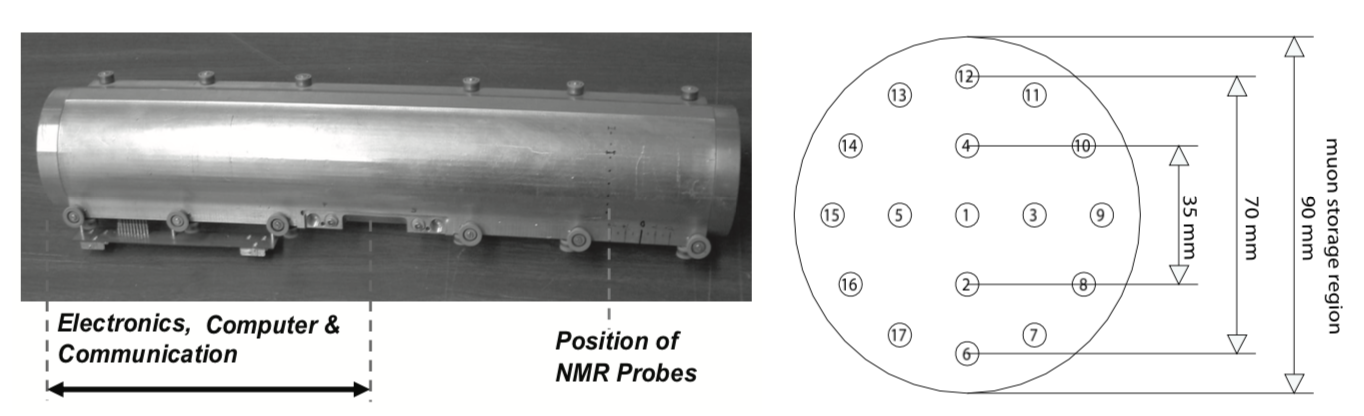
\includegraphics[scale=0.6]{Figures/trolleypic}
\decoRule
\caption{On the left a photograph of the trolley used to measure the magnetic field in the muon storage region. On the right the layout of the 17 NMR probes in the trolley face.}
\label{fig:trolleypic}
\end{figure}

The magnetic field measurement is carried out by extracting the magnetic field in terms of the free proton Larmor precession frequency $\omega{_p}$. However, the protons from pNMR are in hydrocarbon molecules and covered by other probe material and as such are not free protons. This means that the proton experiences a perturbed magnetic field. An absolute calibration is required to make corrections for these perturbations. This correlates the measured magnetic field with the Larmor precession frequency of a free proton and must be done for each trolley probe at every location it measures. This is carried out using two NMR probes; the absolute calibration probe and the plunging probe. The absolute calibration probe measures the field at the same positions as the central trolley probe. This can then be cross calibrated with the plunging probe which also measures the field in the muon storage region \cite{Reference22}.

\section{Detector systems}

\subsection{Calorimeters}

The primary physics goal of the calorimeter is to measure the energy and hit time of decay positrons. The calorimeters record the number of high energy positrons versus time to enable the calculation of $\omega_{a}$. After a muon decays, the positron has insufficient energy to continue its trajectory around the magic radius. Therefore it curls inwards and is incident on a calorimeter.

\begin{figure}[th]
\centering
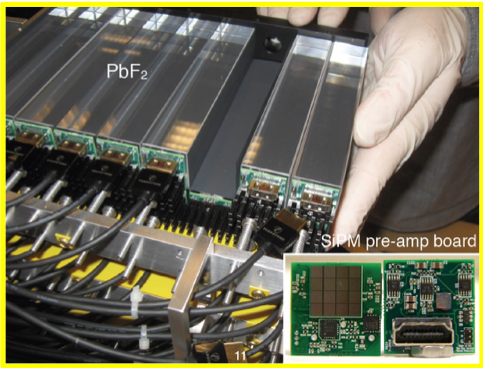
\includegraphics[scale=1.4]{Figures/calorimeterphoto}
\decoRule
\caption{Photograph of a calorimeter crystals being installed.}
\label{fig:calorimeterphoto}
\end{figure}

The experiments calorimeter system contains 24 calorimeter stations equally spaced on the inside radius of the magnetic storage ring \cite{Reference24}. Each of these calorimeters is made up of 54 Lead Fluoride (PbF2) crystals distributed in an array of 6 crystals high and 9 crystals wide. A photograph of calorimeter crystals being installed is shown in figure 4.9. PbF2 crystals were selected due to their fast Cherenkov light signal and good energy resolution. Each crystal is 255 mm wide, 25 mm tall and 140 mm deep \cite{calref1}.

Once inside the crystals, decay positrons produce particle showers. Cerenkov light passes downstream through the crystal and is detected and readout at the edge of the crystal by a silicon photo multiplier (SiPM). Each crystal is separately wrapped in highly reflective Millipore paper to reduce this light from passing into neighbouring crystals. SiPM detectors act as pixelated Geiger counters. As photons hit a pixel, the subsequent avalanche is summed up with all other pixel hits to create an overall signal. Quenching resistors are also relied upon to bring a halt to an avalanche. A pixels recovery time is of the order of a few 10 ns with unaffected pixels already able to receive a pulse. The design relied upon the fact that the number of pixels outnumbered the highest photon count that the crystal would receive.

The calorimeters requirements are:

$\bullet$ The reconstructed positron energy summed together from all calorimeter segments needs to be better than 5$\%$ at 2 GeV. 

$\bullet$ For positrons with kinetic energy above 100 MeV the hit time determined from the SiPM current pulse must have a timing resolution of less that 100 ps.

$\bullet$ The calorimeters are required to have 100$\%$ efficiency in resolving two showers with a time separation of more than 5 ns. For two showers which have a time difference less than this, the calorimeters are required to resolve 66$\%$ of these occasions \cite{Reference22}.

A laser calibration system is used to monitor and calibrate the gain variation of each crystal and SiPM \cite{calref2}\cite{calref3}. To do this laser pulses are continually fired to each calorimeter during and between certain muon fills. This enables the correction of any changes in the gain observed. Out of fill pulses are also fired and used to correct for long term drifts in the calorimeter performance due to temperature effects.

\subsection{Fiber beam monitors}

The Fiber beam monitors are constructed from scintillating fibers. These detectors provide a measurement of the stored muon beam distribution and associated beam dynamics parameters. However the fiber beam monitors carry out a destructive measurement and so are not used during data taking. They can be inserted into and retracted from the storage region as needed.
\begin{figure}[th]
\centering
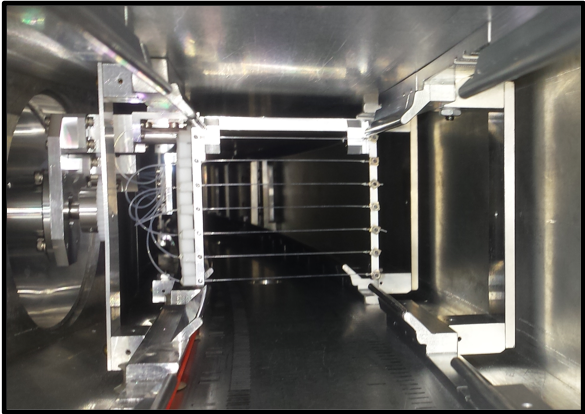
\includegraphics[scale=1.2]{Figures/fiberharpphoto}
\decoRule
\caption{Photograph of a fiber harp in the muon beam storage region.}
\label{fig:fiberharpphoto}
\end{figure}

Every fiber harp monitor contains seven scintillating fibers which are 90 mm long, 0.5 mm in diameter each separated by 13 mm to create a harp like structure. There are four fiber harps placed inside the storage ring, two placed at 180$^{\circ}$ and two at 270$^{\circ}$. At both locations, one fiber harp is orientated so that its fibers are vertical and the other horizontal to measure both the radial and vertical beam profiles. The latter of which is shown in figure 4.10. The fiber harps can also be rotated horizontally. This is done so that all the fibers will measure the same beam and as such can be used for calibration \cite{fiberref1}.

\subsection{Straw tracking detectors}

The straw tracking detectors are designed to make non-destructive measurements of the stored muon profile throughout the duration of each muon fill by measurement of decay positrons. Two tracking stations are placed at 180$^{\circ}$ and 270$^{\circ}$ around the inside of the ring, each directly upstream of a calorimeter. At these locations around the ring, when a decay positron travels inwards to the centre of the storage ring it can pass through straw tracker modules. The positrons pass through the individual straws ionising the gas and creating a pulse, then travel onwards to be detected by a calorimeter. Tracks of the positrons path can then be made by fitting the individual straw hits and this can be extrapolated back to the point of the muon decay. From this the muon beam profile can be built. A detailed description of the straw trackers will be given in chapter 5.

\subsection{Inflector beam monitoring system}

The inflector beam monitoring system (IBMS) is used to determine the muon beam distribution as it's injected into the storage ring. It continuously measures the time the beam enters the storage ring, the intensity of the beam and its XY profiles. Examples of which are shown in figures 4.11 and 4.12. This information is used to determine how to efficiently store the muon beam, leading to better data acquisition and more precise results. 

IBMS detectors determine how the injection beam optics tune is correlated with muon beam storage and beam dynamics properties. The injection of muons into the storage ring can then be optimised by altering the beam tune to ensure the maximum number of stored muons. The IBMS contains three detectors positioned upstream of the storage ring. These detectors are made from scintillating fibers which are read out by SiPMs. The detectors are situated both upstream and downstream of the inflector and downstream of the magnet yoke hole \cite{ibmsref1}\cite{ibmsref2}.  

\begin{figure}[!h]
	\centering
	\begin{minipage}[t]{11cm}
		\centering
		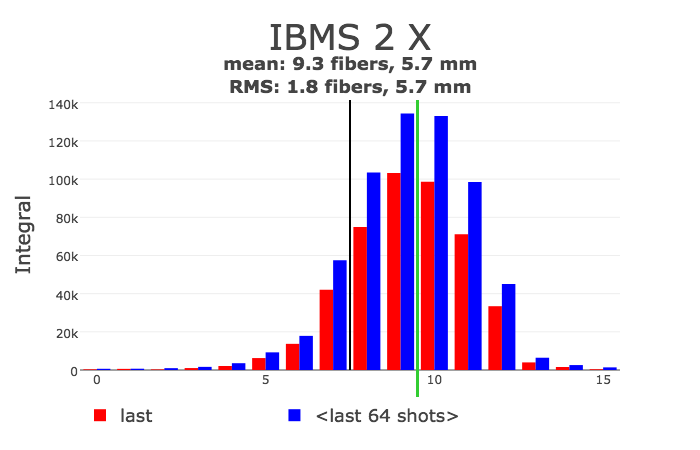
\includegraphics[scale=0.5]{Figures/IBMS2_X_DQM.png}
		\caption{A data quality monitoring plot of the X profile of an IBMS signal.}
	\end{minipage}
	\hspace{3cm}
	\begin{minipage}[t]{11cm}
		\centering
		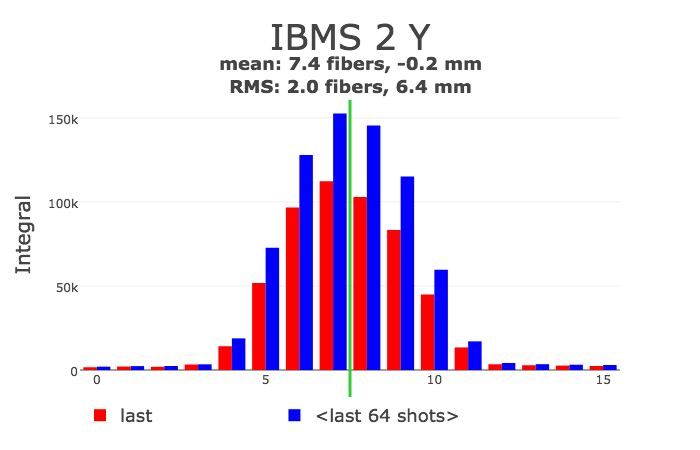
\includegraphics[scale=0.5]{Figures/IBMS2_Y_DQM.png}
		\caption{A data quality monitoring plot of the Y profile of an IBMS signal.}
	\end{minipage}
	\end{figure}

There is also a scintillator detector called the entrance counter. This is placed at the entrance to the storage ring to record the injection time of a fill (T0). The T0 is used to set the injection time for all of the detectors, with the convention that each fill starts at 0 at the start of a T0 pulse. An example of a T0 waveform is shown in figure 4.13. This is required to align data from multiple fills, which helps to avoid the smearing of the $\omega_{a}$ signal\cite{Reference22}.

\begin{figure}[th]
\centering
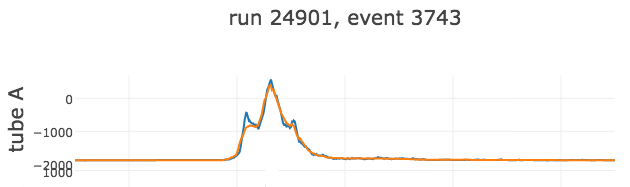
\includegraphics[scale=0.7]{Figures/t0plot.png}
\decoRule
\caption{A data quality monitoring plot displaying a T0 waveform. The orange line showing the average of the last 4 fills and the blue is showing the waveform from the previous fill.}
\label{fig:t0plot}
\end{figure}
